PostgreSQL là một hệ quản trị cơ sở dữ liệu quan hệ với mã nguồn mở mạnh mẽ, sử dụng và mở rộng ngôn ngữ SQL, kết hợp với nhiều tính năng giúp lưu trữ và xử lí khối dữ liệu hiệu quả nhất. PostgreSQL ra đời năm 1986 như một phần của dự án POSTGRES tại Đại học California (Berkeley) và đã có hơn 30 năm phát triển tích cực trên nền tảng cốt lõi.\par

PostgreSQL đã tạo được danh tiếng mạnh mẽ nhờ kiến trúc, độ tin cậy, tính toàn vẹn của dữ liệu, bộ tính năng mạnh mẽ, khả năng mở rộng và sự đóng góp của cộng đồng mã nguồn mở đằng sau để liên tục cung cấp các giải pháp hiệu quả và sáng tạo. PostgreSQL chạy trên tất cả các hệ điều hành chính, tuân thủ ACID từ năm 2001 và có các tiện ích bổ sung mạnh mẽ như bộ mở rộng cơ sở dữ liệu không gian địa lý PostGIS. Không có gì ngạc nhiên khi PostgreSQL đã trở thành hệ quản trị cơ sở dữ liệu mã nguồn mở được nhiều người và tổ chức lựa chọn.\par

 \begin{figure}[h!]
    \begin{center}
        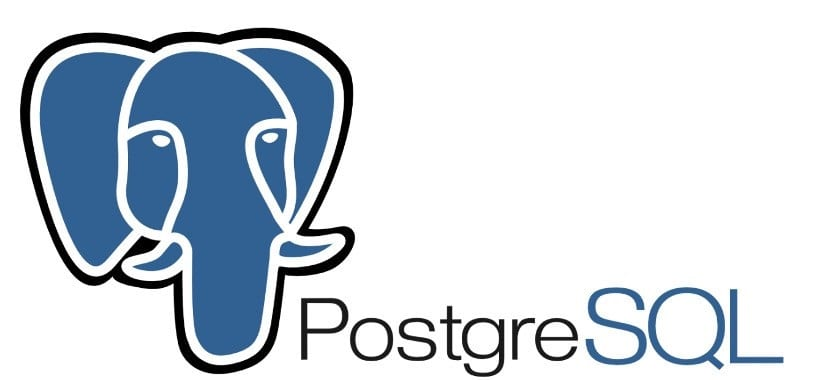
\includegraphics[width=10cm]{Image/Technical/postgresql.png}
        \caption{Postgres Database.}
        \label{postgres}
    \end{center}
\end{figure}

\par
Postgres SQL có những ưu điểm như dưới đây:
\begin{itemize}
    \item Mã nguồn mở và nhẹ.
    \item Dễ sử dụng, sửa đổi và triển khai.
    \item Có khả năng chịu lỗi cao nhờ vào cơ chế ghi nhật kí trước (write-ahead logging - WAL)
    \item Hỗ trợ các đối tượng địa lý để có thể sử dụng nó cho các dịch vụ dựa trên vị trí và hệ thống thông tin địa lý.
    \item Cộng đồng sử dụng lớn mạnh.
\end{itemize}
Bên cạnh đó Postgres SQL ccũng có các nhược điểm:
\begin{itemize}
    \item Hiệu suất thực hiện các toán tử đơn giản kém hơn so với các hệ quản trị cơ sở dữ liệu quan hệ khác như MySQL, Oracle,... Nhưng đối với toán tử phức tạp thì tốt hơn rất nhiều.
    \item Do vẫn còn là một hệ quản trị cơ sở dữ liệu mới nên vẫn chưa được hỗ trợ một cách đầy đủ nhất.
\end{itemize}